\documentclass[10pt,landscape]{article}
\usepackage{multicol}
\usepackage{calc}
\usepackage{ifthen}
\usepackage[landscape]{geometry}
\usepackage{amsmath,amsthm,amsfonts,amssymb}
\usepackage{color,graphicx}
\usepackage{hyperref}
\usepackage[font=scriptsize,labelfont=bf]{caption}
\usepackage{wrapfig}
\usepackage{graphicx,calc}
%\usepackage{pbox}

\pdfinfo{
  /Title (Leistungelektronik)
  /Creator (TeX)
  /Producer (pdfTeX 1.40.0)
  /Author (Noah Huetter)
  /Subject (Leistungelektronik)
  /Keywords (Leistungelektronik,ETH)}

% This sets page margins to .5 inch if using letter paper, and to 1cm
% if using A4 paper. (This probably isn't strictly necessary.)
% If using another size paper, use default 1cm margins.
\ifthenelse{\lengthtest { \paperwidth = 11in}}
    { \geometry{top=.5in,left=.5in,right=.5in,bottom=.5in} }
    {\ifthenelse{ \lengthtest{ \paperwidth = 297mm}}
        {\geometry{top=1cm,left=1cm,right=1cm,bottom=1cm} }
        {\geometry{top=1cm,left=1cm,right=1cm,bottom=1cm} }
    }

% Turn on simple page number
\pagestyle{plain}

% Redefine section commands to use less space
\makeatletter
\renewcommand{\section}{\@startsection{section}{1}{0mm}%
                                {-1ex plus -.5ex minus -.2ex}%
                                {0.5ex plus .2ex}%x
                                {\normalfont\large\bfseries}}
\renewcommand{\subsection}{\@startsection{subsection}{2}{0mm}%
                                {-1explus -.5ex minus -.2ex}%
                                {0.5ex plus .2ex}%
                                {\normalfont\normalsize\bfseries}}
\renewcommand{\subsubsection}{\@startsection{subsubsection}{3}{0mm}%
                                {-1ex plus -.5ex minus -.2ex}%
                                {1ex plus .2ex}%
                                {\normalfont\small\bfseries}}
\makeatother

% make smaller enumerates
\usepackage{enumitem}
\setlist[enumerate]{itemsep=-1mm,leftmargin=3mm}

% Define BibTeX command
\def\BibTeX{{\rm B\kern-.05em{\sc i\kern-.025em b}\kern-.08em
    T\kern-.1667em\lower.7ex\hbox{E}\kern-.125emX}}

% Don't print section numbers
\setcounter{secnumdepth}{0}


\setlength{\parindent}{0pt}
\setlength{\parskip}{1pt plus 0.5ex}

%My Environments
\newtheorem{example}[section]{Example}
% -----------------------------------------------------------------------
\newcommand{\eqn}[3]
{
  \begin{minipage}[#1]{#2}
    \[ #3 \]
  \end{minipage}
}
\newcommand{\feqn}[3]
{
\fbox{
  \begin{minipage}[#1]{#2}
    \[ #3 \]
  \end{minipage}
}
}
 

 
\begin{document}


\raggedright
\footnotesize
\begin{multicols}{2}



% multicol parameters
% These lengths are set only within the two main columns
%\setlength{\columnseprule}{0.25pt}
\setlength{\premulticols}{1pt}
\setlength{\postmulticols}{1pt}
\setlength{\multicolsep}{1pt}
\setlength{\columnsep}{2pt}

\begin{center}
     \Large{\underline{Leistungelektronik}} \\
\end{center}
% -----------------------------------------------------------------------
\IfFileExists{../build/revision.tex}{
  \input{../build/revision.tex}
  Author: Noah Huetter \hfill Date: \compiledate \hspace{1em} Commit: \revision
}{Author: Noah Huetter}


% -----------------------------------------------------------------------
\vspace{2mm}\hrule
\section{Allgemein}
\eqn{h}{0.23\linewidth}{ i_L(t) = \frac{1}{L}\int u_L(t)dt }
\eqn{h}{0.23\linewidth}{ u_L(t) = L\frac{d}{dt}i_L(t) }
\eqn{h}{0.23\linewidth}{ i_C(t) = C\frac{d}{dt}u_C(t) }
\eqn{h}{0.23\linewidth}{ u_C(t) = \frac{1}{C}\int i_C(t)dt }


\eqn{h}{0.15\linewidth}{ Q=C\cdot U }

\eqn{h}{0.23\linewidth}{ V_{rms} = \sqrt{ \frac{1}{T} \int_T u^2(t)dt } }
\eqn{h}{0.23\linewidth}{V_{rms,sin} = \hat{V} / \sqrt{2}} \eqn{h}{0.23\linewidth}{V_{rms,pwm} = \hat{V} \sqrt{D}}

% -----------------------------------------------------------------------
\vfill\null
\columnbreak
\vspace{2mm}\hrule
\section{Tiefsetzsteller}

\begin{center}
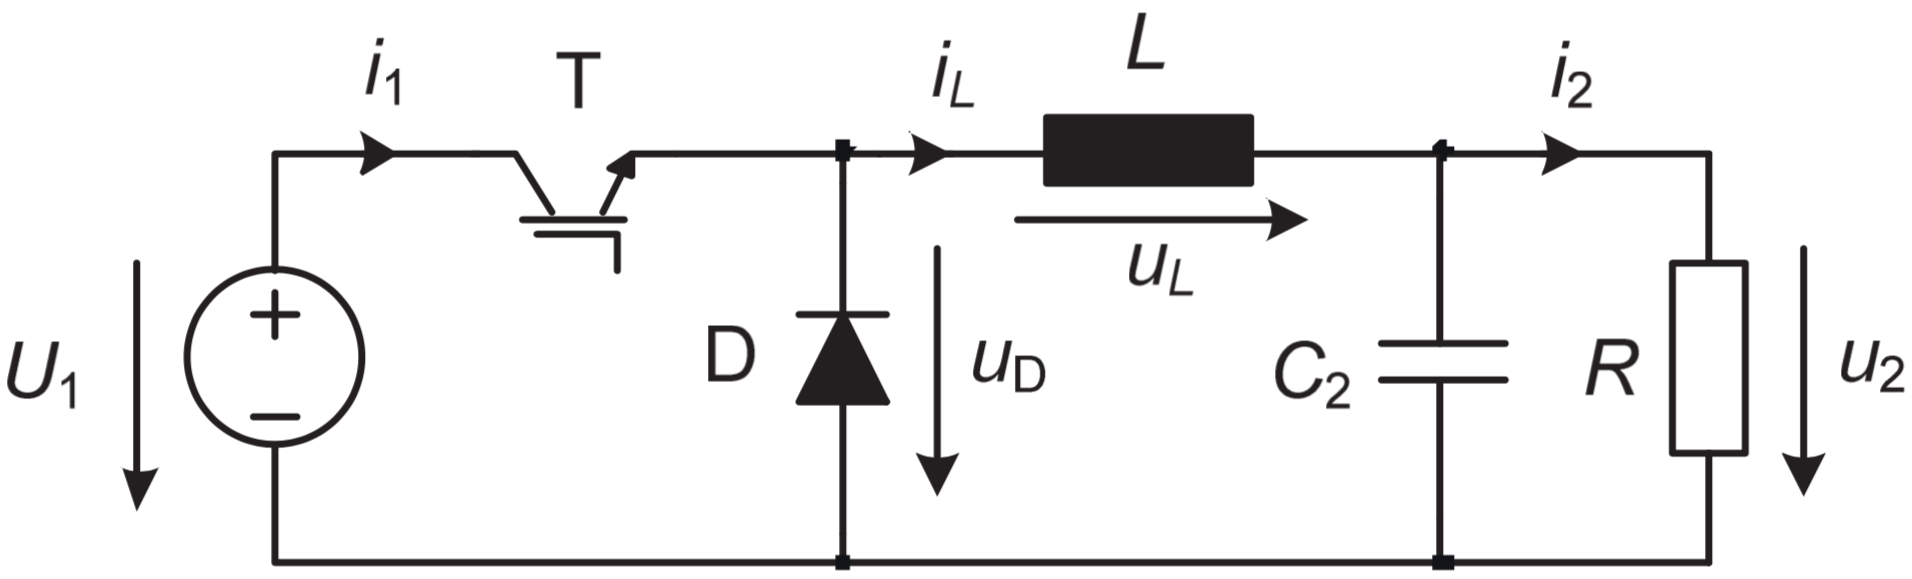
\includegraphics[width=0.8\linewidth]{img/sch_buck.png}%
\captionof{figure}{Tiefsetzsteller}%
\end{center}

\subsection{Kontinuierlicher Stromfluss}

\begin{tabular}{c c}
  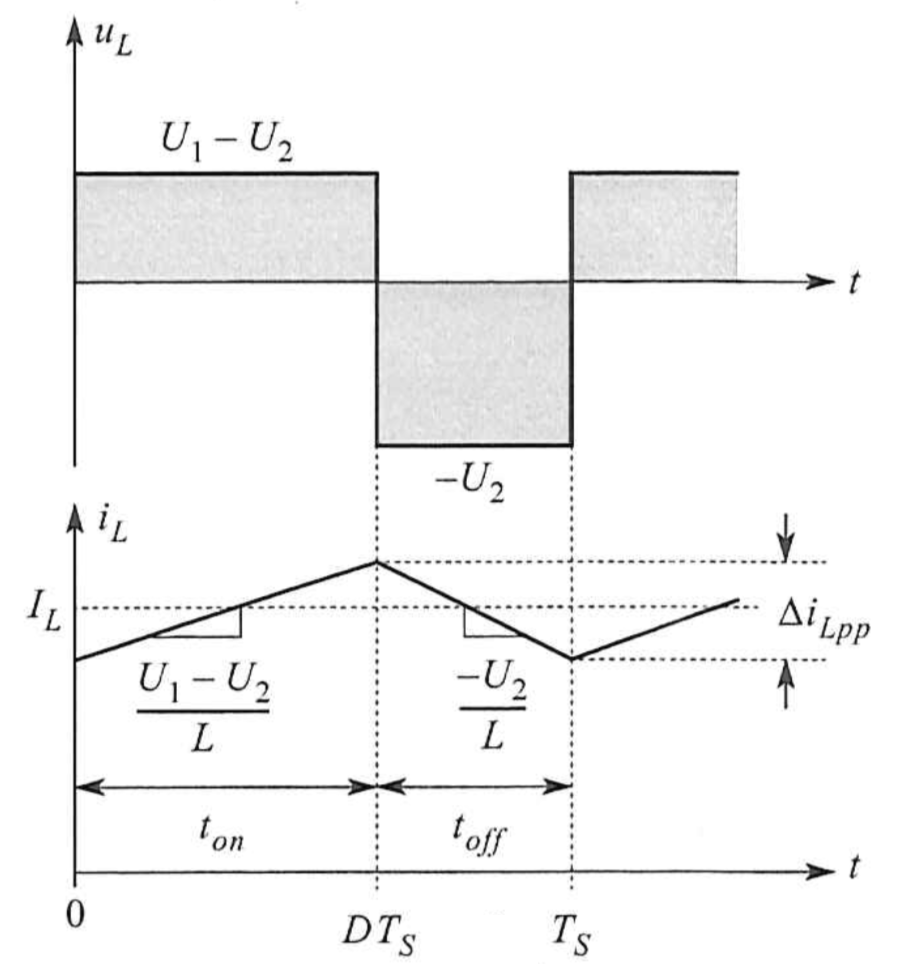
\includegraphics[width=0.4\linewidth]{img/buck/cont.png}%
  &
  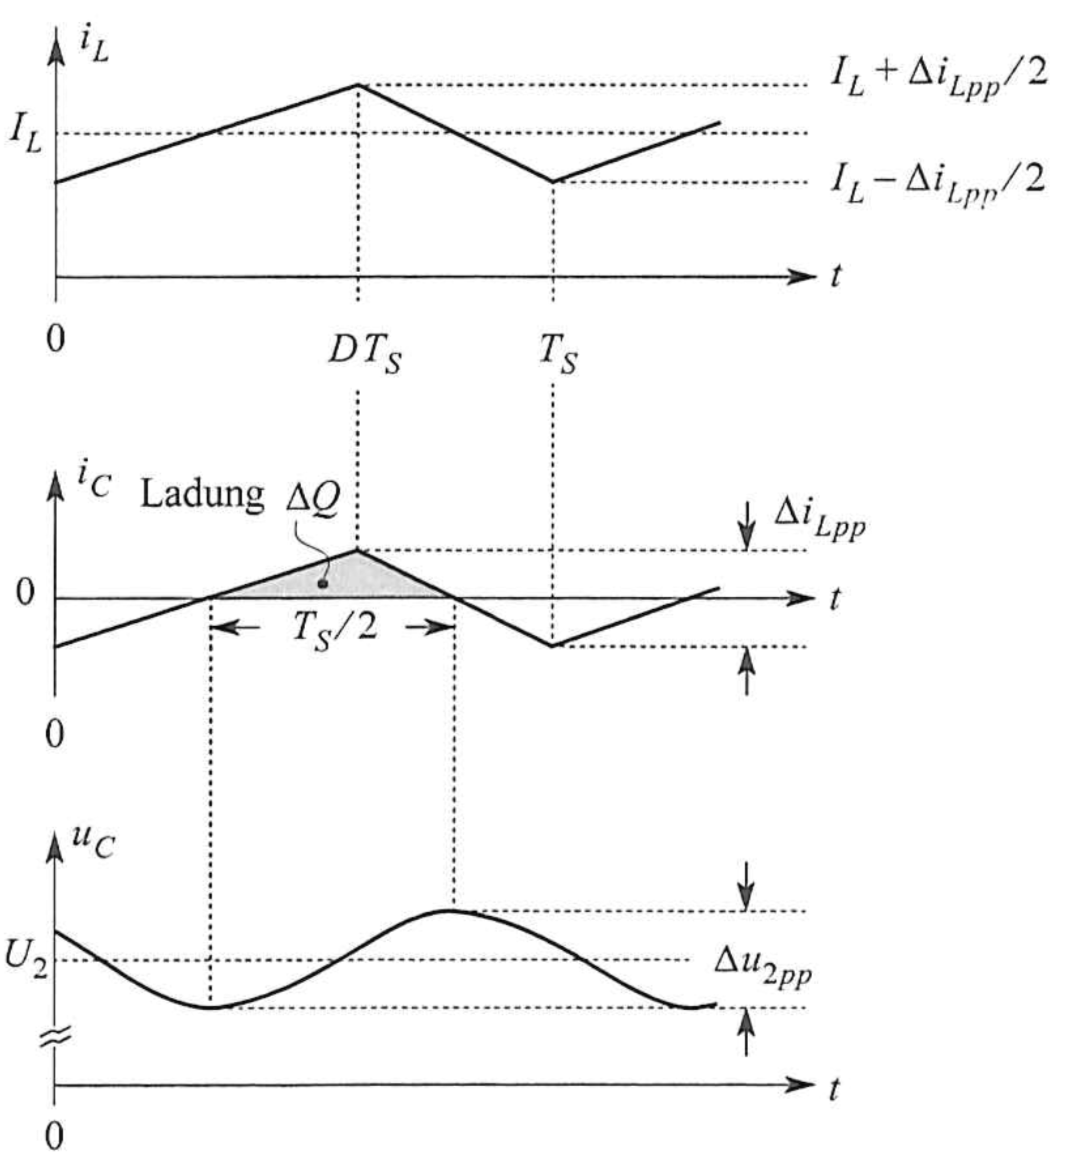
\includegraphics[width=0.4\linewidth]{img/buck/out.png}%
\end{tabular}

\eqn{h}{0.25\linewidth}{ D = \frac{I_1}{I_2} = \frac{U_2}{U_1} }
\eqn{h}{0.25\linewidth}{ \Delta i_{Lpp} = \frac{U_2}{L}(1-D)T_S}
\eqn{h}{0.25\linewidth}{ \Delta u_{2pp}=\Delta U_C = \frac{U_2}{L}(1-D) T_S \frac{T_S}{8 \cdot C}}

\subsection{Diskontinuierlicher Stromfluss}
\begin{tabular}{c c}
  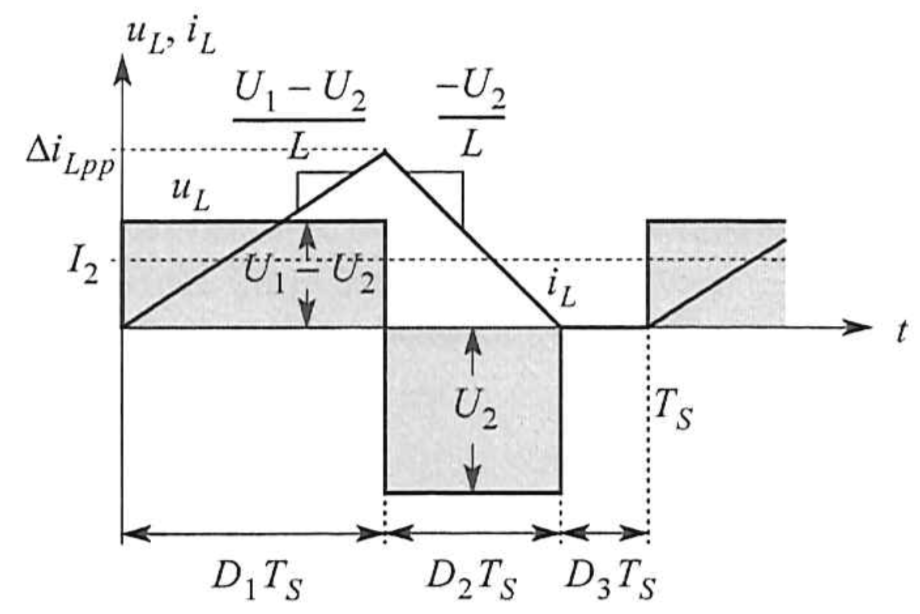
\includegraphics[width=0.4\linewidth]{img/buck/discont.png}%
  &
  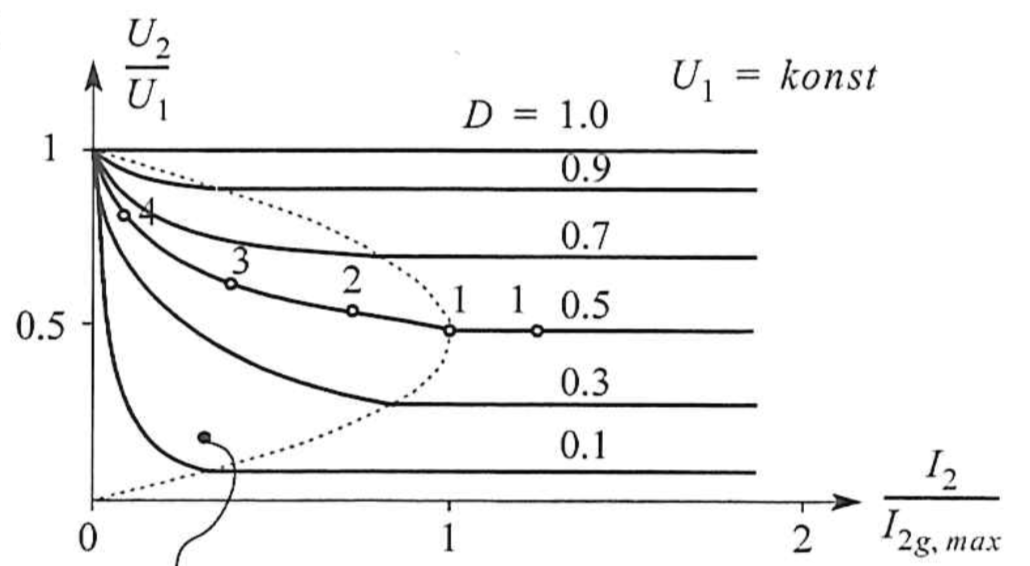
\includegraphics[width=0.4\linewidth]{img/buck/discplot.png}%
\end{tabular}

\eqn{h}{0.4\linewidth}{ I_{2g} = \frac{1}{2} \Delta i_{Lpp} = \frac{U_2}{2 \cdot L}(1-D)T_S}
\eqn{h}{0.25\linewidth}{ R_{g} = \frac{2L}{(1-D) \cdot T_S}}
\eqn{h}{0.25\linewidth}{ U_2=U_1 \frac{D_1}{D_1+D_2} }
\eqn{h}{0.3\linewidth}{ I_{2g,max}=I_{2g}|_{D=0.5} = \frac{U_1 T_S}{8L} }
\eqn{h}{0.3\linewidth}{ \frac{U_2}{U_1}=\frac{D^2}{D^2+\frac{1}{4} \frac{I_2}{I_{2g,max}} } }
\eqn{h}{0.25\linewidth}{ D = \frac{1}{2} \sqrt{\frac{I_2/I_{2g,max}}{U_1/U_2-1}} }

% -----------------------------------------------------------------------
\vfill\null
\columnbreak
\vspace{2mm}\hrule
\section{Hochsetzsteller}

\begin{center}
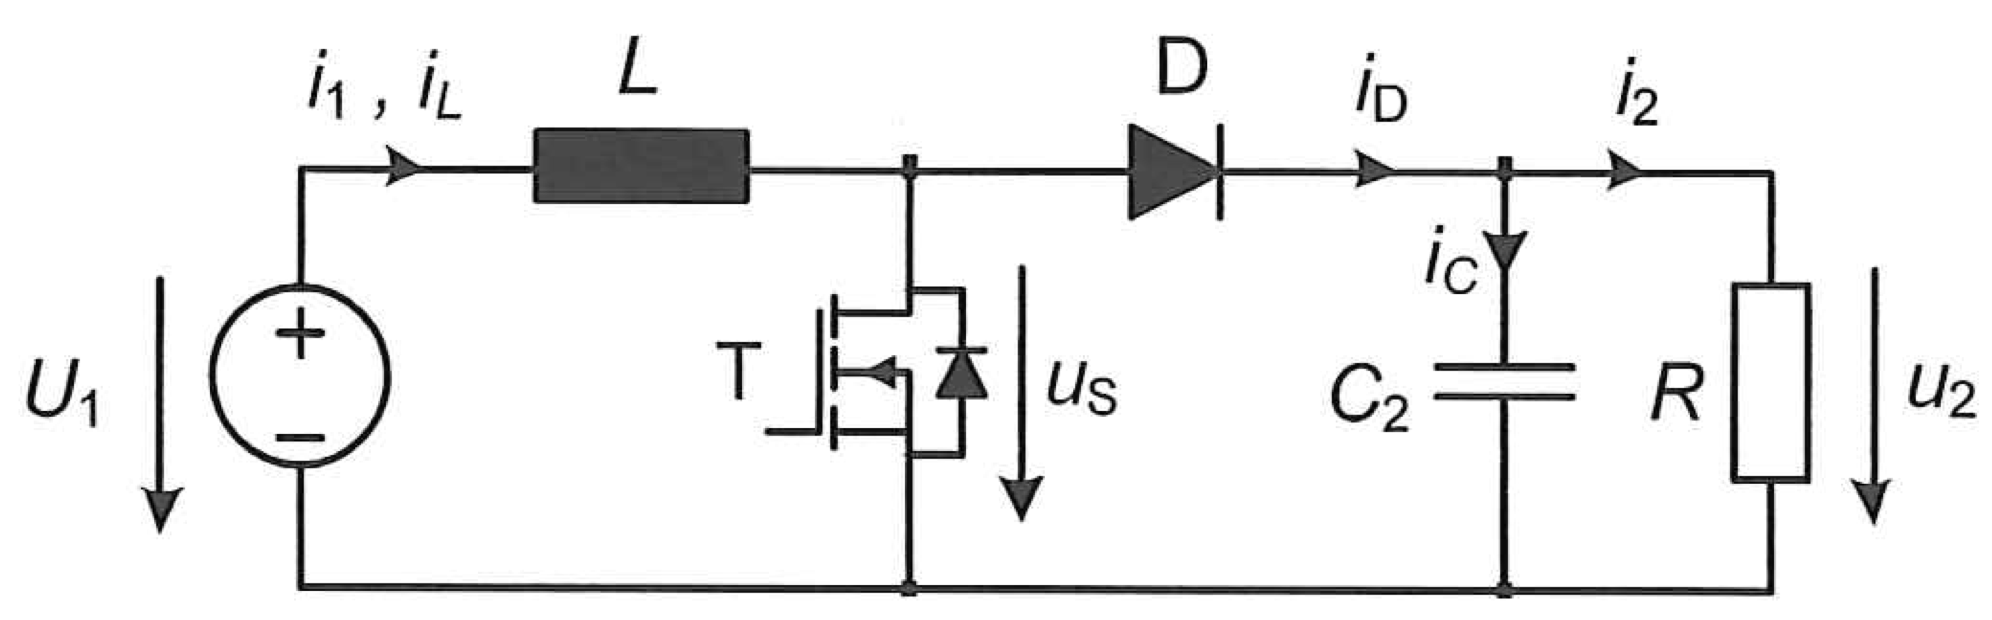
\includegraphics[width=0.8\linewidth]{img/sch_boost.png}%
\captionof{figure}{Hochsetzsteller}%
\end{center}

\subsection{Kontinuierlicher Stromfluss}
\eqn{h}{0.23\linewidth}{ D = 1 - \frac{U_1}{U_2} }
\eqn{h}{0.23\linewidth}{ \frac{U_2}{U_1} = \frac{1}{1-D}}
\eqn{h}{0.23\linewidth}{ \frac{I_2}{I_1}=1-D }
\eqn{h}{0.23\linewidth}{ \Delta i_{Lpp} = \frac{U_1}{L}DT_S}

\eqn{h}{0.23\linewidth}{ \Delta U_{2pp} = \frac{U_2}{R}\frac{DT_s}{C_2} }

\subsection{Diskontinuierlicher Stromfluss}
\eqn{h}{0.3\linewidth}{ I_{Lg} = \frac{1}{2} \frac{(U_2-U_1)}{L}(1-D)T_s }
\eqn{h}{0.3\linewidth}{ I_{2g} = \frac{1}{2} \frac{U_2}{L}D(1-D)^2T_s }
\eqn{h}{0.3\linewidth}{ I_{2g,max} = I_{2g}|_{D=1/3} = \frac{2}{27}\frac{U_2}{L}T_S }

\eqn{h}{0.3\linewidth}{ D= \sqrt{\frac{4}{27}\frac{U_2}{U_1} \left (\frac{U_2}{U_1}-1 \right ) \frac{I_2}{I_{2g,max}} } }
\eqn{h}{0.3\linewidth}{ I_{1g} = \frac{1}{2} \frac{U_2}{L}D(1-D)T_s }

% \eqn{h}{0.25\linewidth}{ }
% -----------------------------------------------------------------------
\vfill\null
\columnbreak
\vspace{2mm}\hrule
\section{Tief-Hochsetzsteller}

\begin{center}
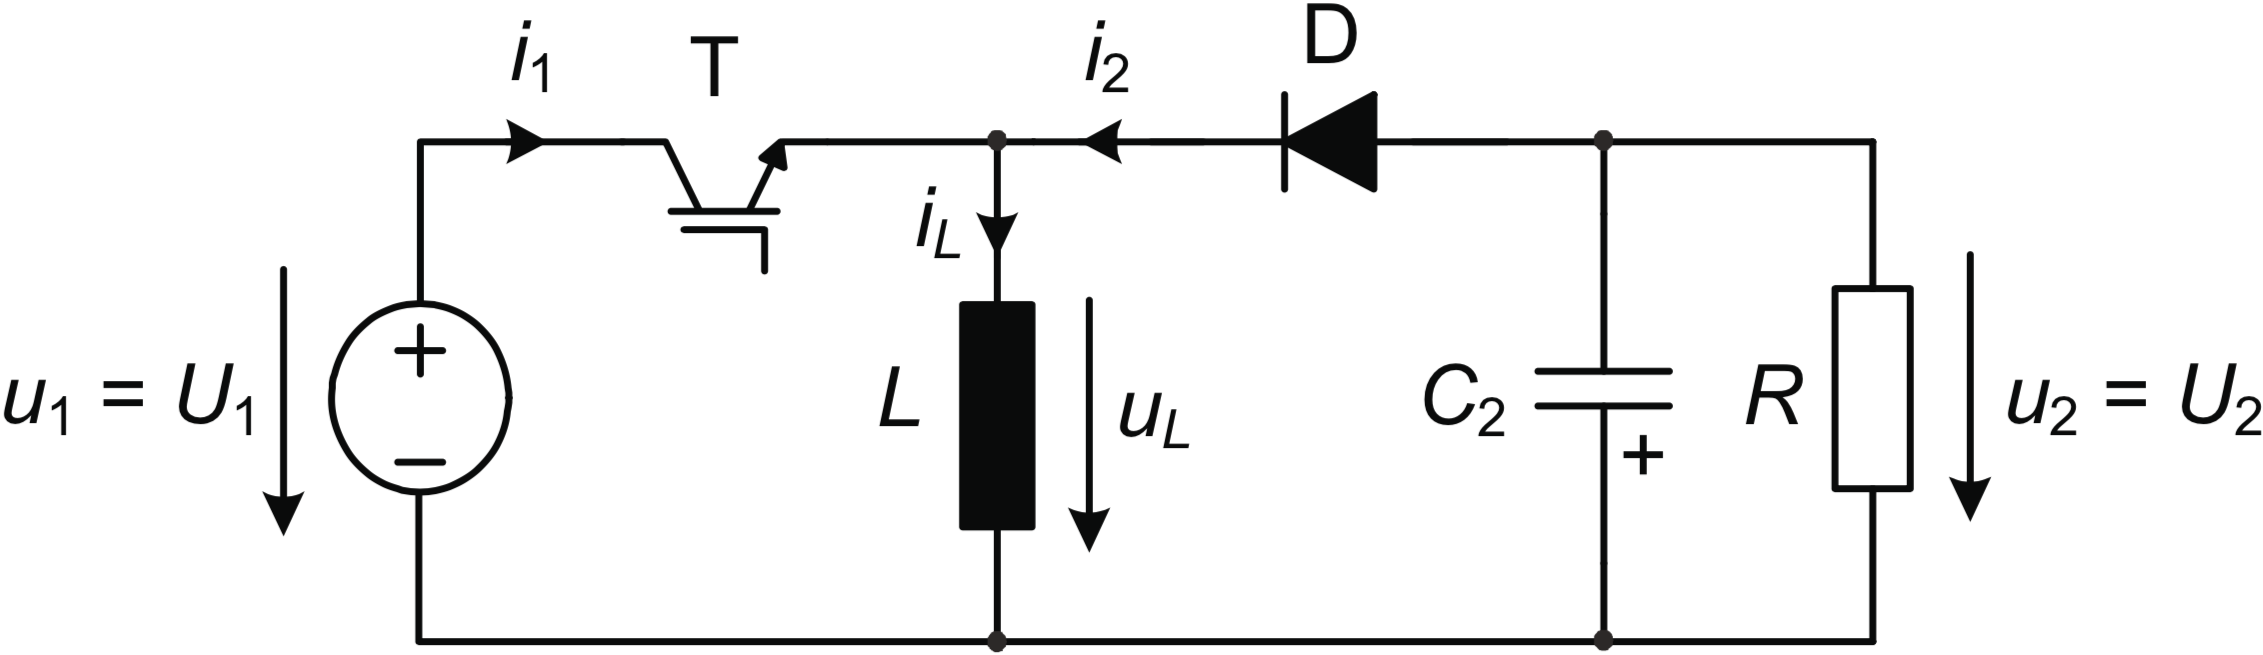
\includegraphics[width=0.8\linewidth]{img/sch_invers.png}%
\captionof{figure}{Tief-Hochsetzsteller}%
\end{center}

\subsection{Kontinuierlicher Stromfluss}
\eqn{h}{0.23\linewidth}{ \frac{U_2}{U_1} = -\frac{D}{1-D} }
\eqn{h}{0.23\linewidth}{ D = \frac{U_2}{U_2 - U_1} }
\eqn{h}{0.23\linewidth}{ \frac{I_2}{I_1}=\frac{1-D}{D} }

\subsection{Diskontinuierlicher Stromfluss}
\eqn{h}{0.3\linewidth}{ I_{Lg} = \frac{1}{2} \frac{-U_2}{L}(1-D)T_s }
\eqn{h}{0.3\linewidth}{ I_{2g} = \frac{1}{2} \frac{-U_2}{L}(1-D)^2T_s }
\eqn{h}{0.3\linewidth}{ I_{2g,max} = -\frac{1}{2} \frac{U_2}{L}T_s }

\eqn{h}{0.3\linewidth}{ D = -\frac{U_2}{U_1} \sqrt{\frac{I_2}{I_{2g,max}}} }
\eqn{h}{0.65\linewidth}{ P_2 = E_L f_s = \frac{1}{2}L \cdot i_{Lmax}^2 \cdot f_s = \frac{L}{2} f_s \left( \frac{U_1 D T_s}{L} \right)^2 = \frac{U_1^2D^2}{2L}T_s }


% -----------------------------------------------------------------------
\vfill\null
\columnbreak
\vspace{2mm}\hrule
\section{PFC Einphasen Gleichrichter}

\begin{center}
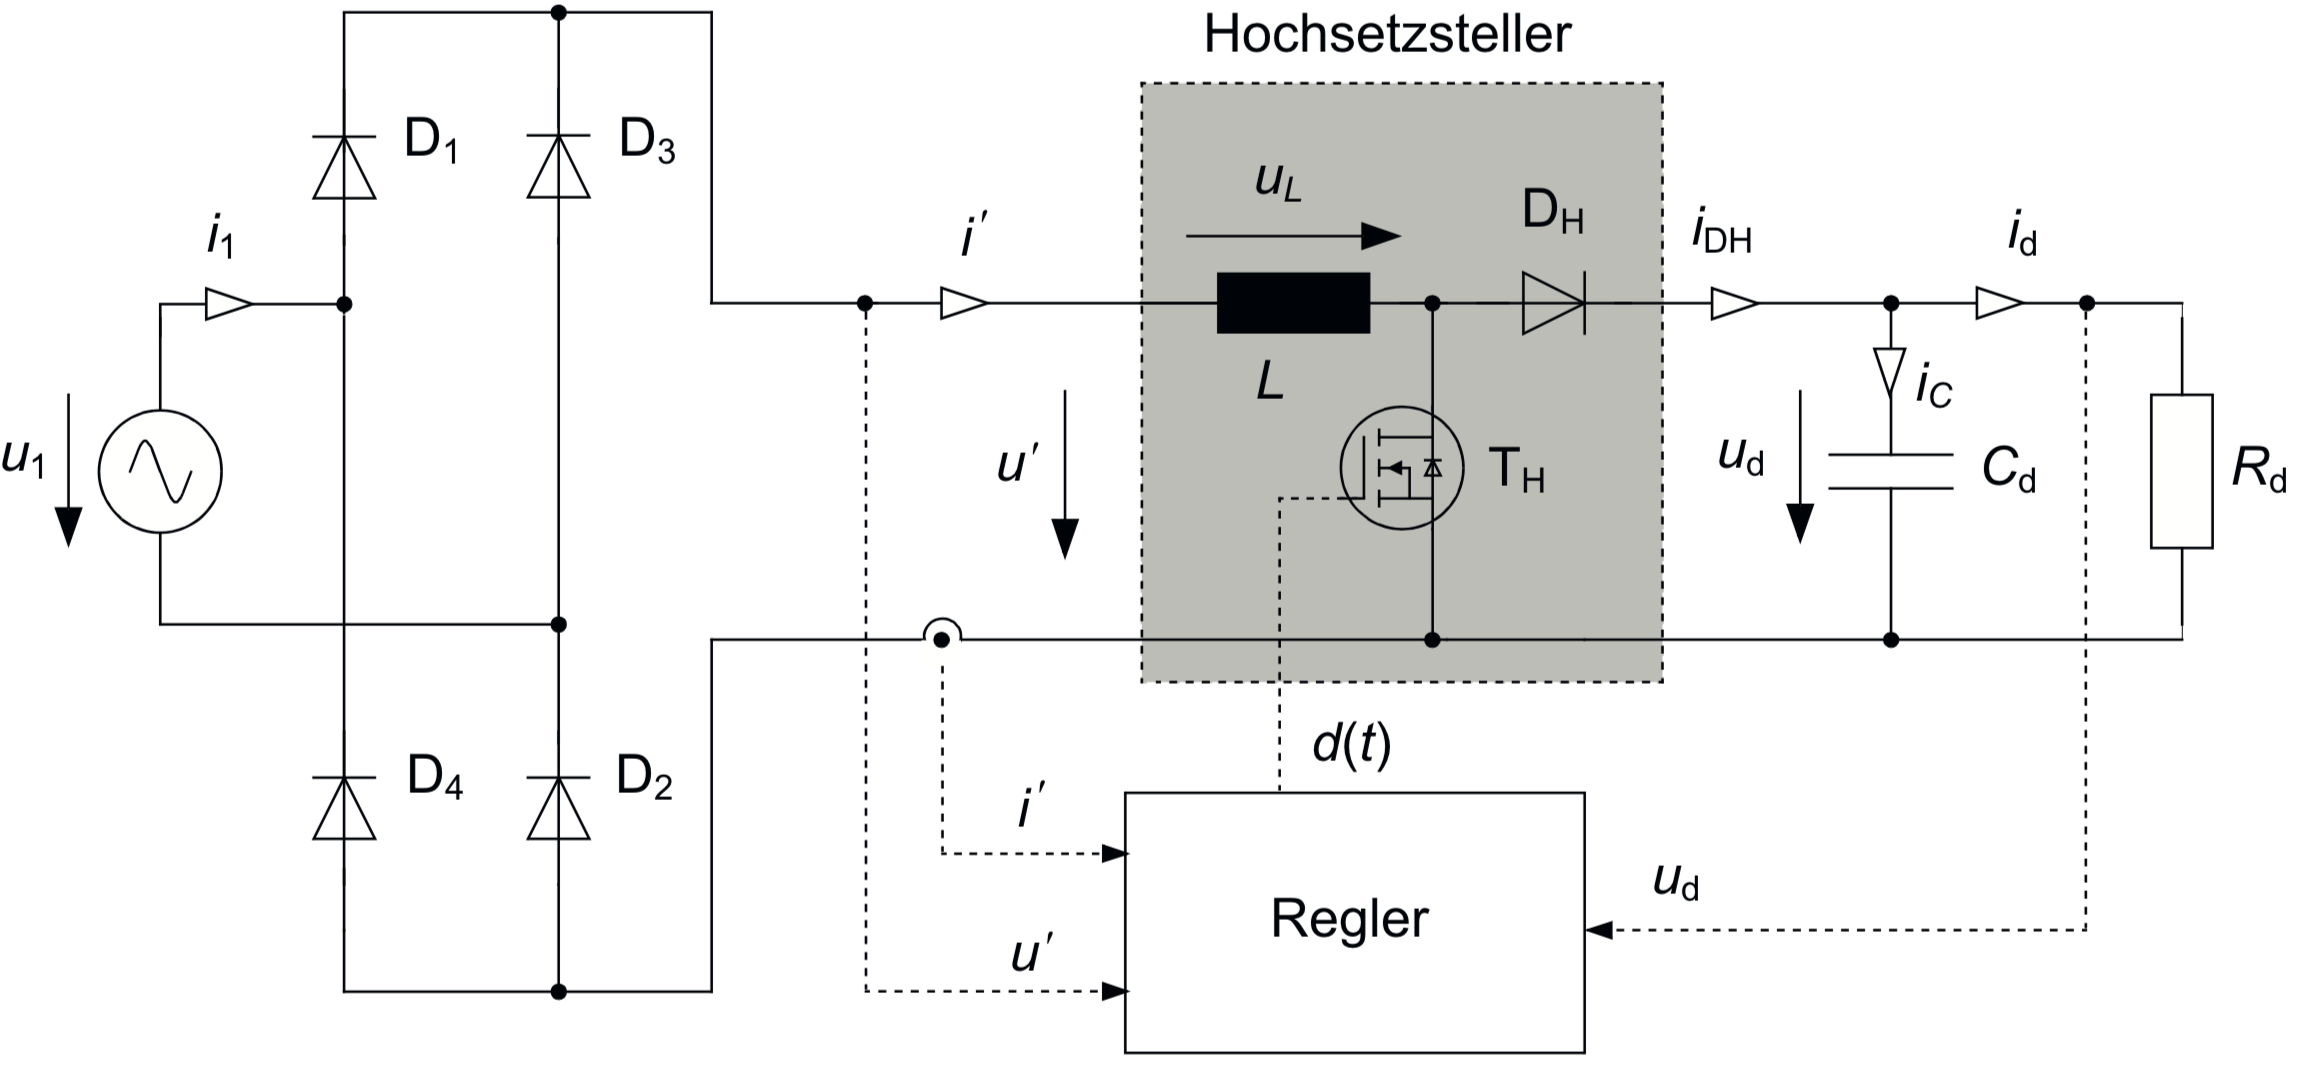
\includegraphics[width=0.8\linewidth]{img/sch_pfc.png}%
\captionof{figure}{PFC Einphasen Gleichrichter}%
\end{center}

\subsection{Toleranzbandregelung}
\eqn{h}{0.23\linewidth}{ i'_{max}=(1+k)i'^* }
\eqn{h}{0.23\linewidth}{ i'_{min}=(1-k)i'^* }
\eqn{h}{0.23\linewidth}{ \Delta i_{pp} = 2k\cdot \hat{i}'^* |sin(\omega t)| }



% -----------------------------------------------------------------------
\vfill\null
\columnbreak
\vspace{2mm}\hrule
\section{Netzgeführte Stromrichter}

\begin{center}
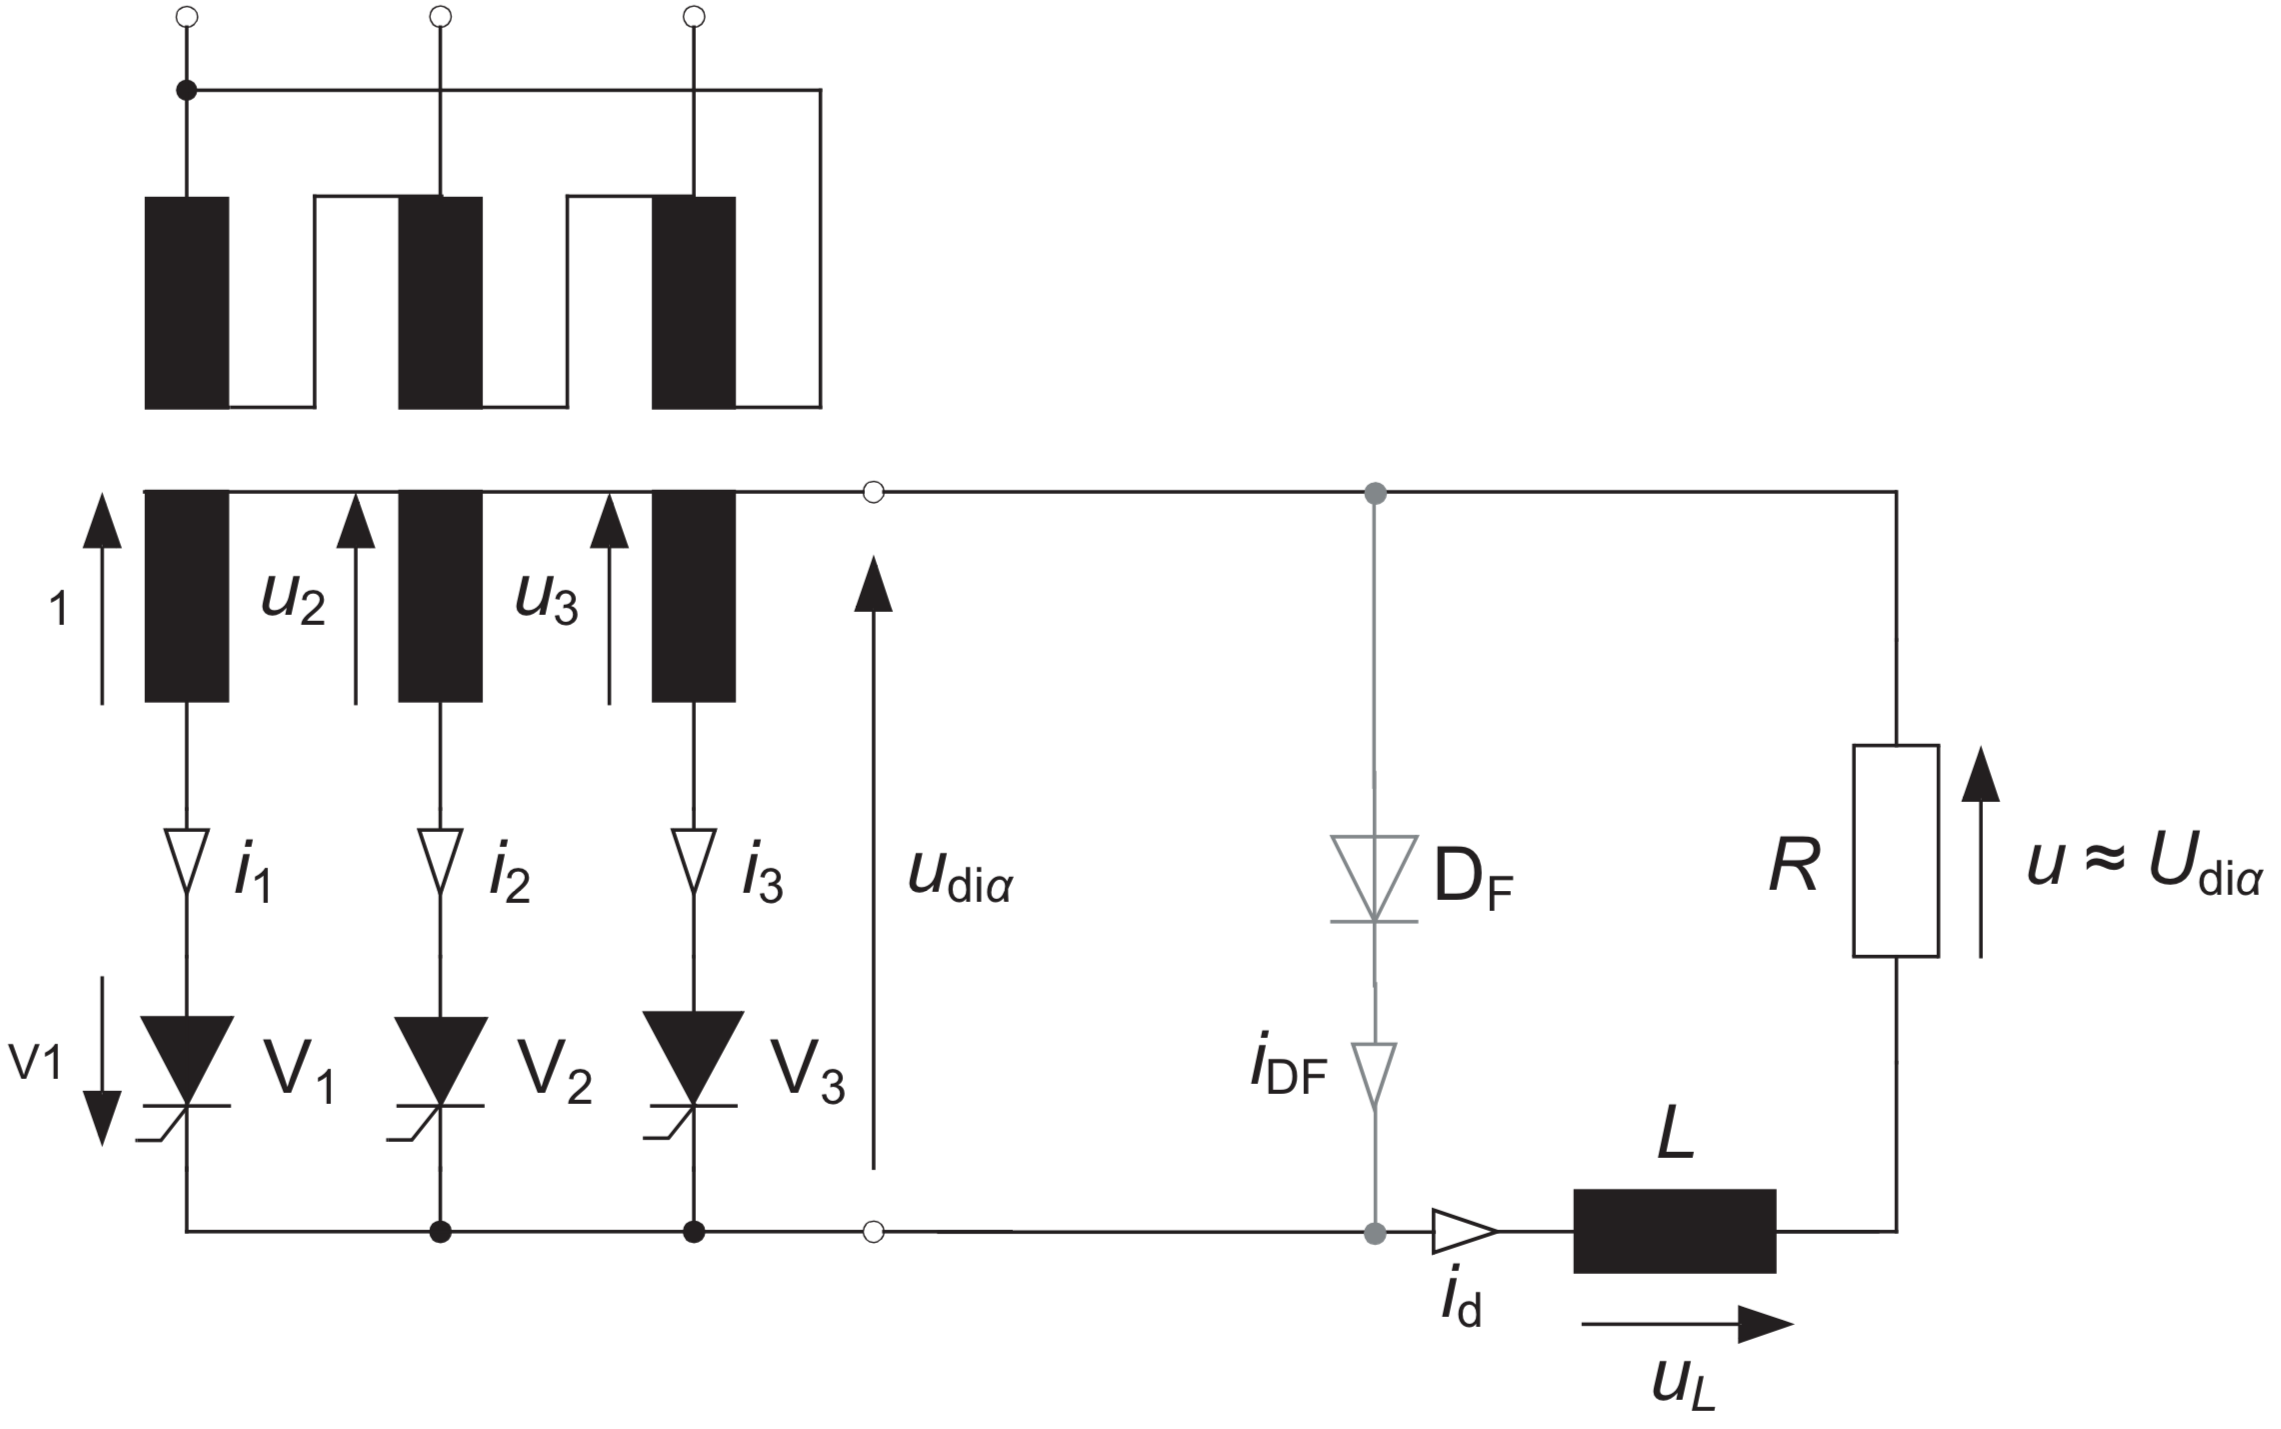
\includegraphics[width=0.8\linewidth]{img/sch_netz_dreiphase.png}%
\captionof{figure}{Dreiphasen netzgeführte Stromrichter}%
\end{center}

Text

% -----------------------------------------------------------------------
\vfill\null
\columnbreak
\vspace{2mm}\hrule
\section{Induktivität Dimensionierung}

\begin{minipage}[h]{0.6\linewidth}
  \begin{tabular}{l l l |}
    $A_n$   & Wicklungsfenster      & $mm^2 = 10^{-6}m^2$ \\
    $A_e$   & Eisenquerschnitt      & $mm^2 = 10^{-6}m^2$ \\
    $B_S$   & Sättigungsinduktion   & $\approx 0.3T$ \\
    $k_f$   & Füllfaktor            & $\approx 0.5$ \\
    $S$     & zulässige Stromdichte & $\approx 5\frac{A}{mm^2}=5\cdot10^6\frac{A}{m^2}$ \\
    $d$     & Luftspalt             & $m$ \\
    $\mu_0$ & Vacuum permeability   & $1.256\cdot10^{-6}Vs/(Am)$
  \end{tabular}
\end{minipage}
\begin{minipage}[h]{0.3\linewidth}
\textbf{Vorgehen}
  \begin{enumerate}
    \item Berechne Flächenprodukt $A_e A_n$
    \item Suche Kern mit grösserem Flächenprodukt
    \item Berechne N
    \item Berechne Luftspalt
  \end{enumerate}
\end{minipage}


\eqn{h}{0.23\linewidth}{ A_e > \frac{L\hat{I}}{B_S N} }
\eqn{h}{0.23\linewidth}{ A_n > \frac{NI_{rms}}{k_f S} }
\eqn{h}{0.23\linewidth}{ A_e A_n = \frac{L \hat{I} I_{rms}}{B_S k_f S} }
\eqn{h}{0.23\linewidth}{ \frac{L \hat{I} }{A_e S} < N < \frac{A_n k_f S}{I_{rms}} }

\eqn{h}{0.23\linewidth}{ A_{cu} S = I_{max} }
\eqn{h}{0.23\linewidth}{ d = \frac{R_{tot}\mu_0 A_e}{2} = \frac{N^2 \mu_0 A_e}{2L} }


% -----------------------------------------------------------------------
\vfill\null
\columnbreak
\vspace{2mm}\hrule
\section{Trafo Dimensionierung}
Text

% -----------------------------------------------------------------------
\vfill\null
\columnbreak
\vspace{2mm}\hrule
\section{Sperrwandler}

\begin{center}
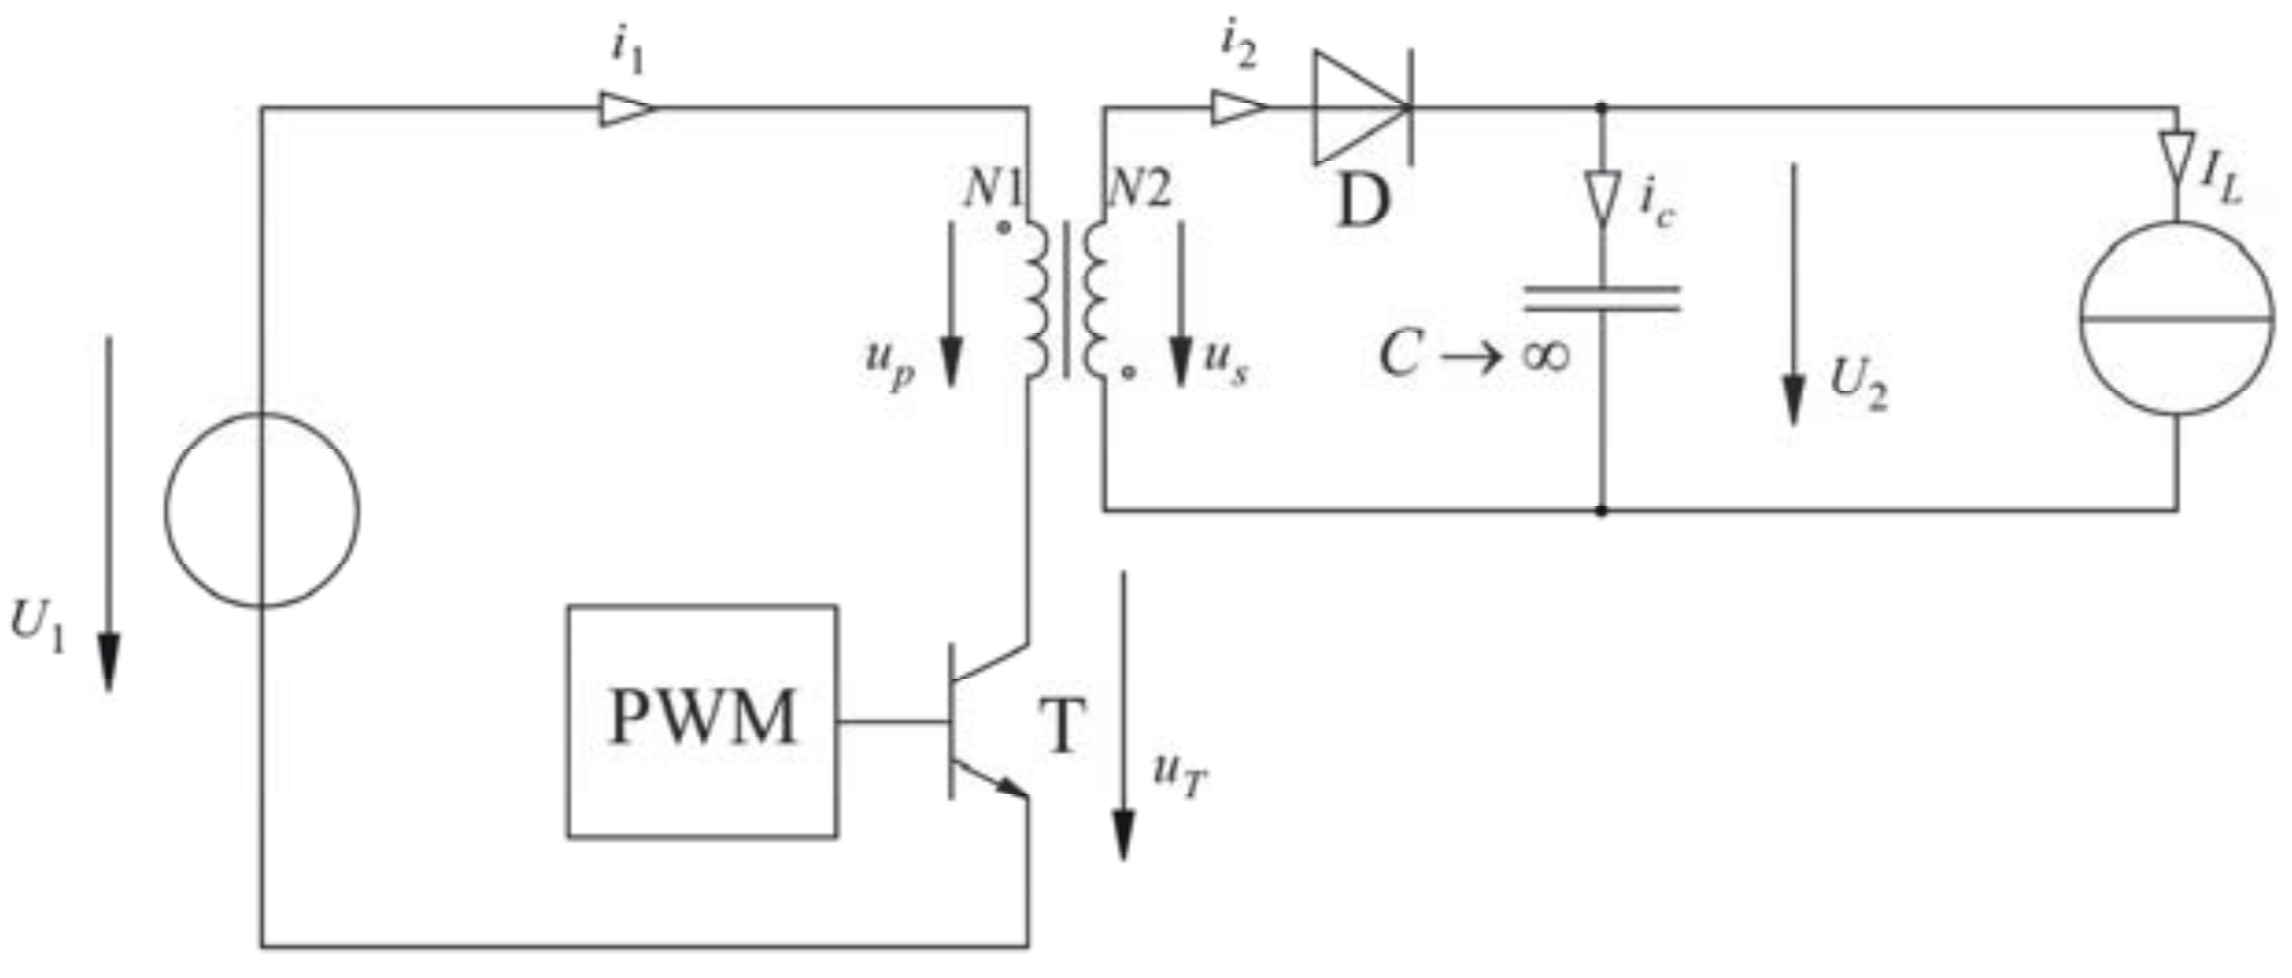
\includegraphics[width=0.8\linewidth]{img/sch_sperr.png}%
\captionof{figure}{Sperrwandler}%
\end{center}

Text

% -----------------------------------------------------------------------
\vfill\null
\columnbreak
\vspace{2mm}\hrule
\section{Durchflusswandler}

\begin{center}
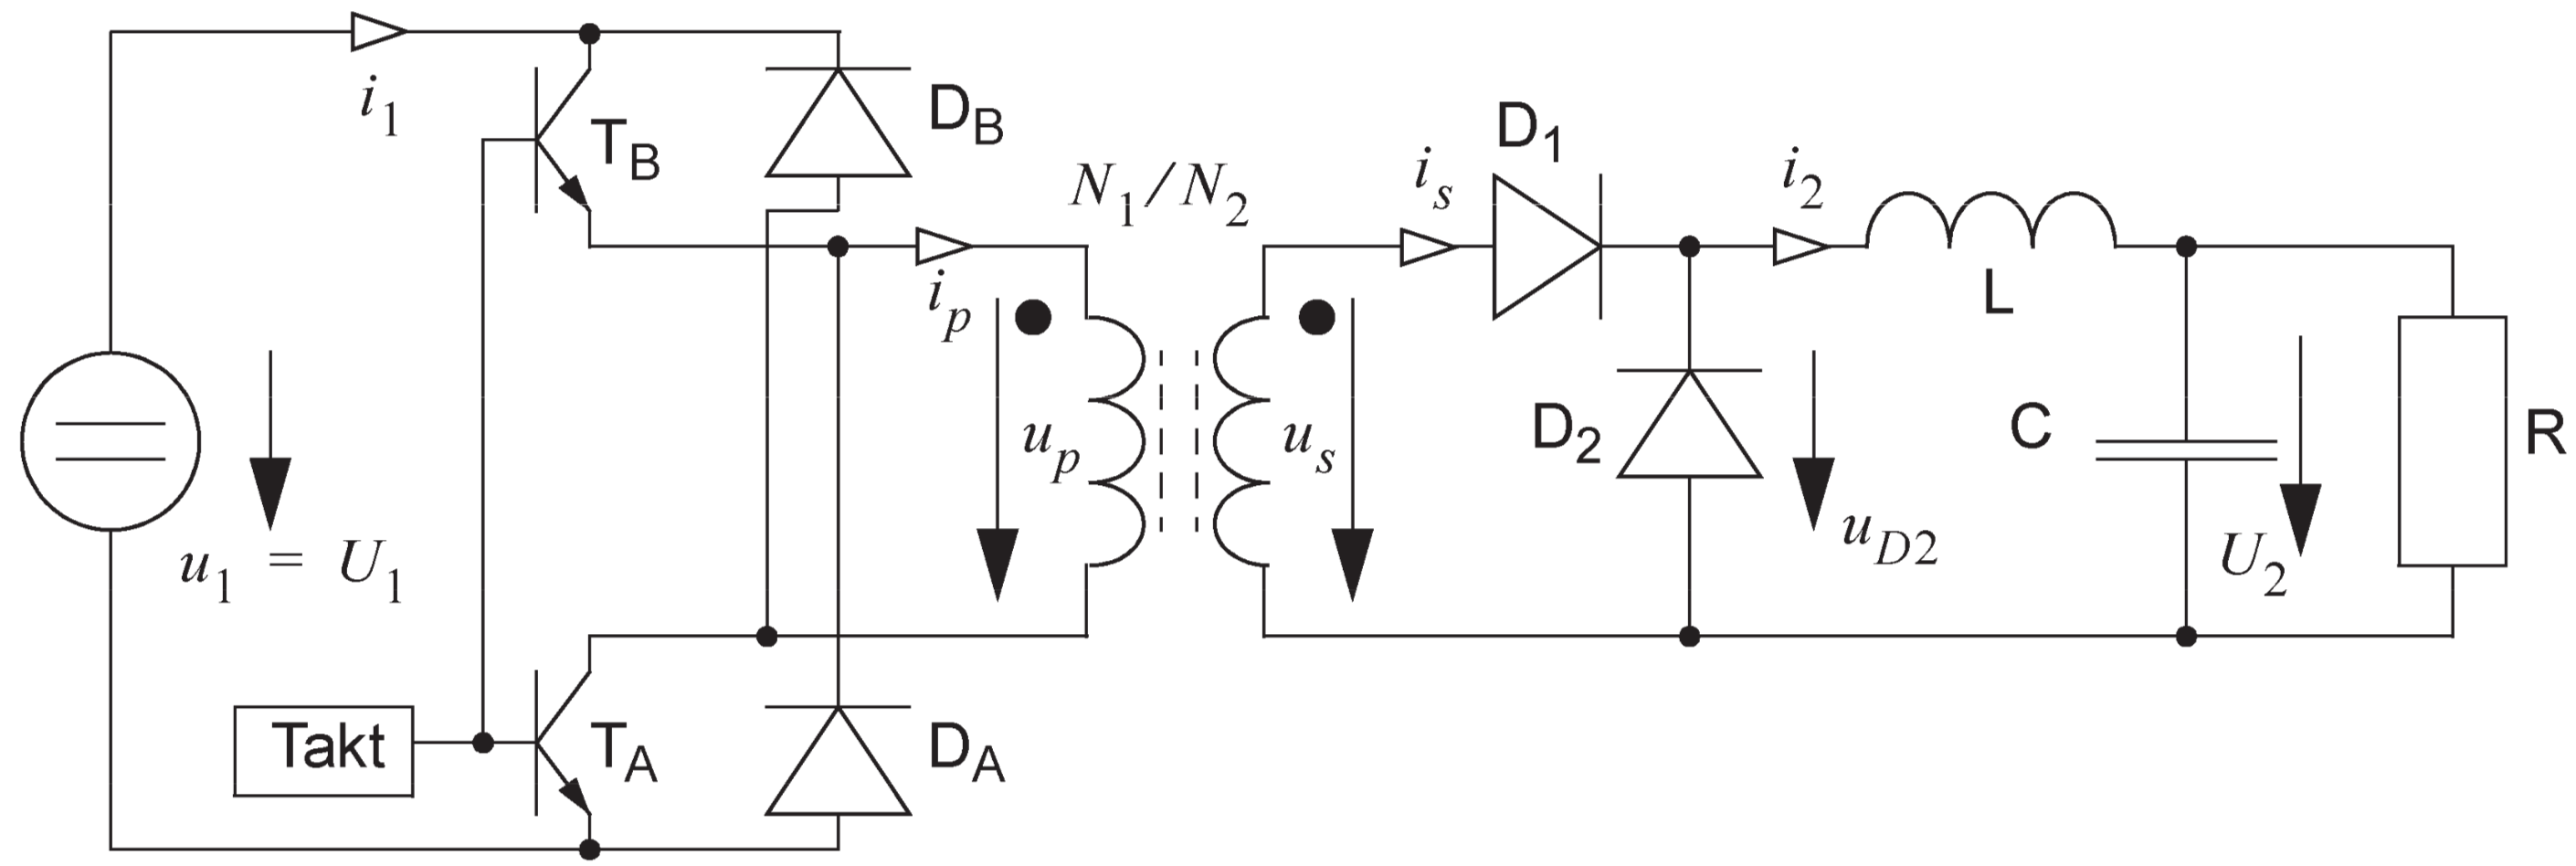
\includegraphics[width=0.8\linewidth]{img/sch_durchfluss.png}%
\captionof{figure}{Zwei-Transistor Durchflusswandler}%
\end{center}

Text

% -----------------------------------------------------------------------
\vfill\null
\columnbreak
\vspace{2mm}\hrule
\section{Einphasen Gleichspannungswechselrichter}

\begin{center}
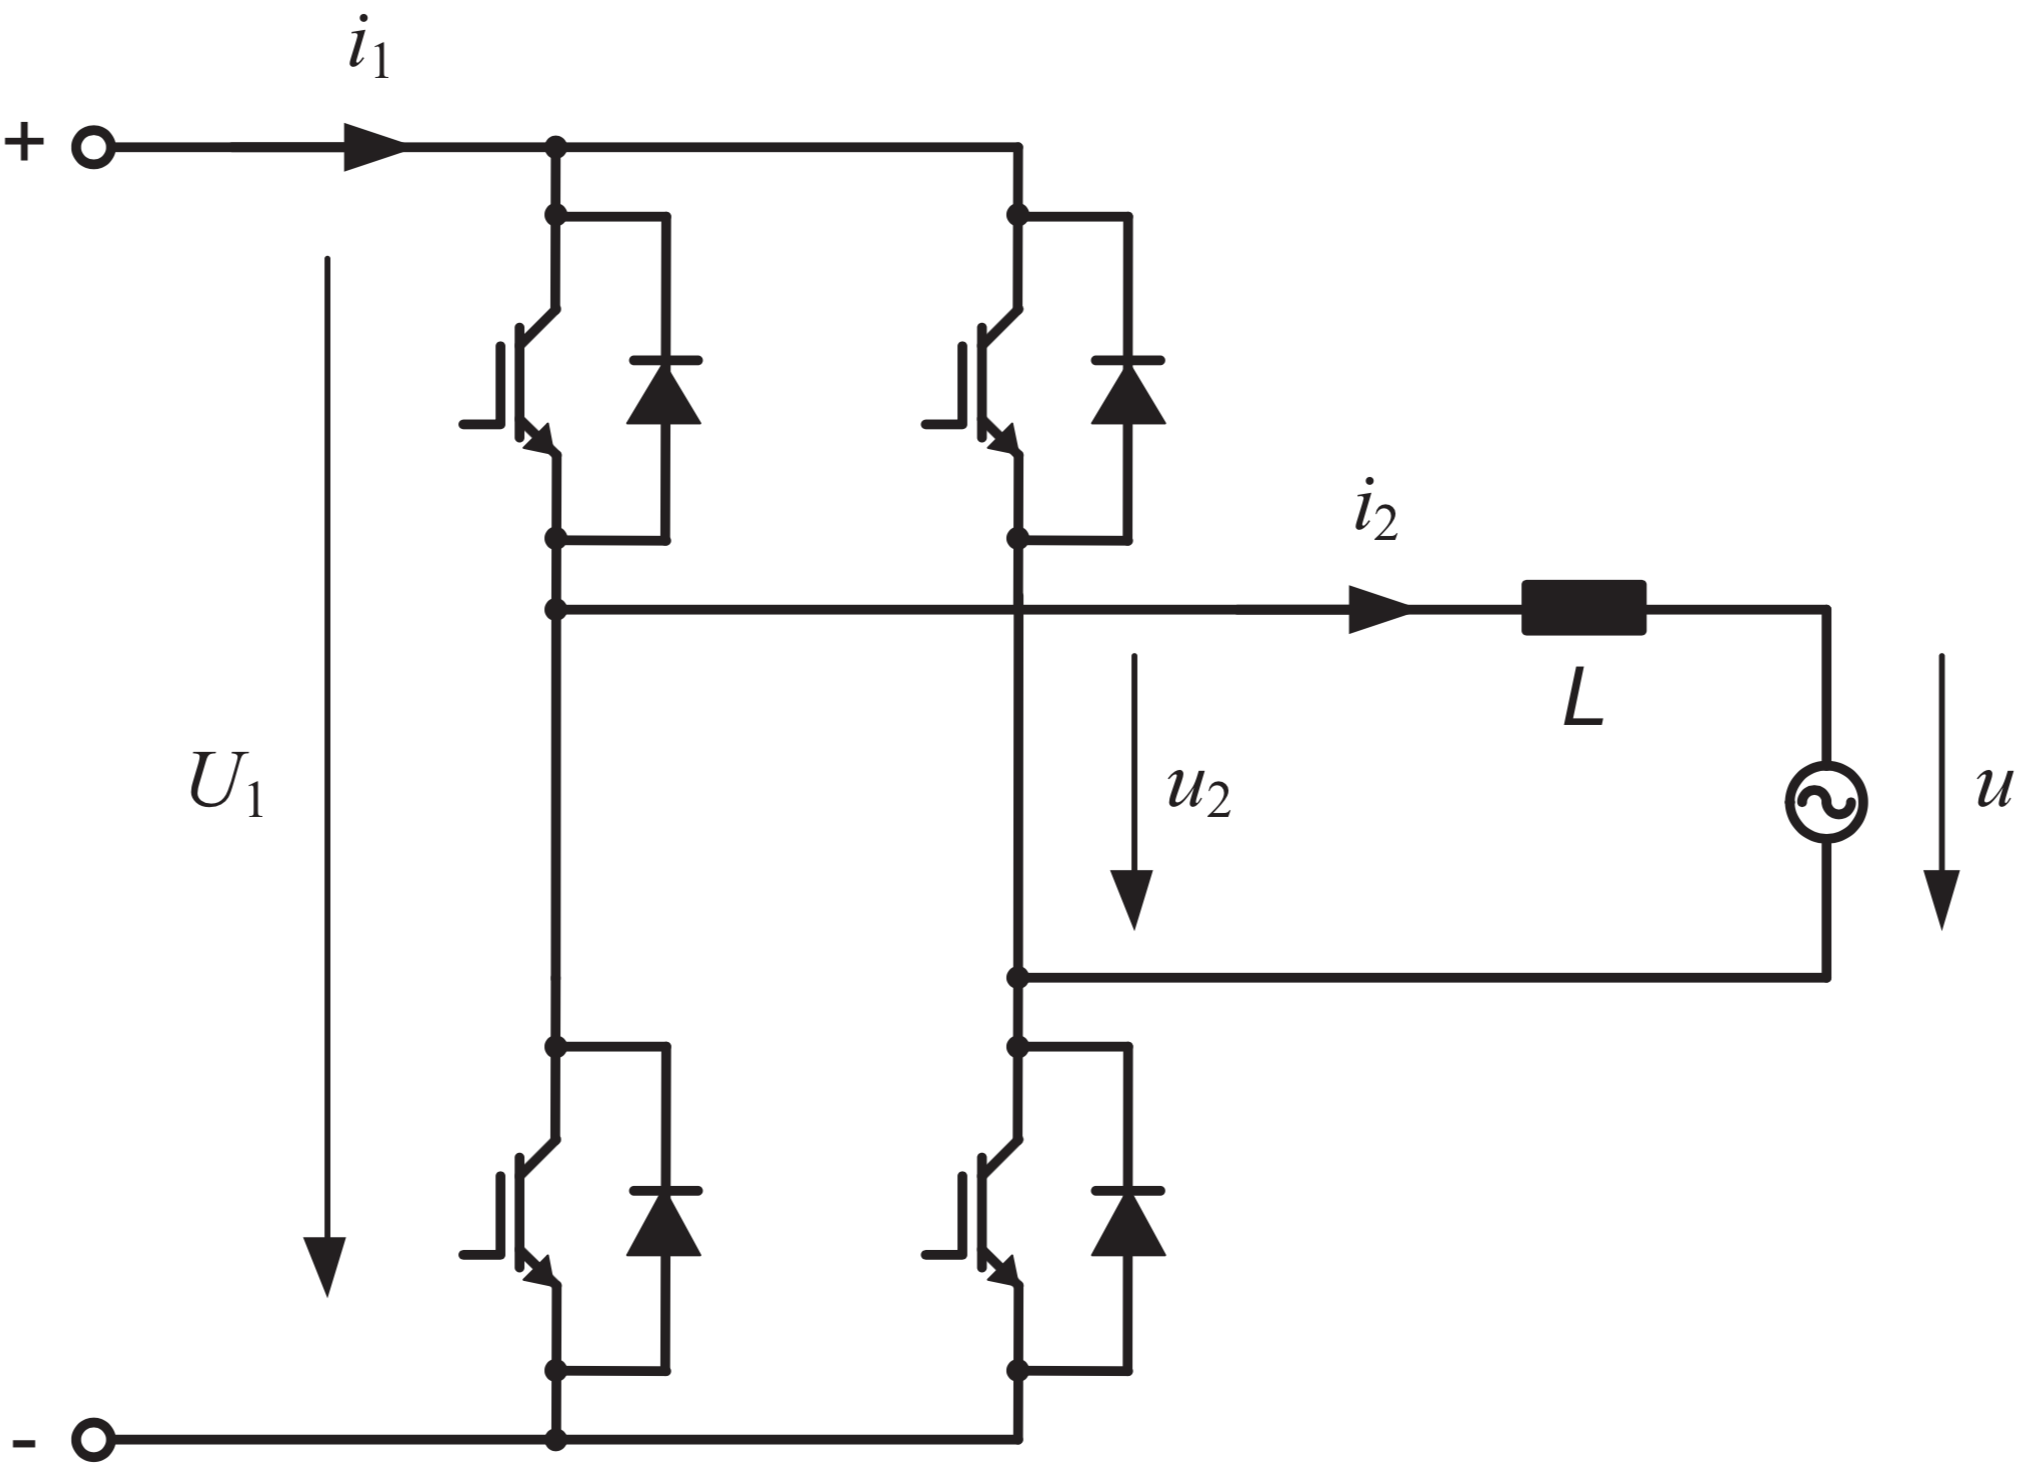
\includegraphics[width=0.8\linewidth]{img/sch_fullbridge.png}%
\captionof{figure}{Einphasiger Gleichspannungswechselrichter}%
\end{center}

Text

% -----------------------------------------------------------------------
\vfill\null
\columnbreak
\vspace{2mm}\hrule
\section{Dreiphasen Gleichspannungswechselrichter}
Text

\clearpage

% You can even have references
\rule{0.3\linewidth}{0.25pt}
%\scriptsize
%\bibliographystyle{abstract}
%\bibliography{refFile}
\end{multicols}
\end{document}
